% =============================================================================
% CAPÍTULO 4 - DISEÑO (COMPLETO, CON BD Y ESTRUCTURA DEL FRONTEND)
% =============================================================================
% Requiere: \usepackage{float}, \usepackage{graphicx}, \usepackage{tikz}
% =============================================================================

\chapter{Diseño}
\label{chap:diseno}

Este capítulo detalla el diseño técnico de la solución propuesta: la arquitectura del sistema, el modelo de datos, la estructura del frontend (capas, rutas e interfaz), el diseño del módulo de inteligencia artificial y las herramientas utilizadas.

% -----------------------------------------------------------------------------
\section{Arquitectura del sistema}
% -----------------------------------------------------------------------------

El sistema sigue una arquitectura cliente-servidor desacoplada, dividida en tres capas principales que garantizan la escalabilidad y el mantenimiento independiente de cada componente.

El \textbf{frontend} está desarrollado con React y TypeScript utilizando Vite como herramienta de construcción. Se organiza en capas (presentación, servicios, contexto y utilidades; véase la sección~\ref{sec:estructura-frontend}). Esta capa se encarga de la interfaz de usuario, gestionando la navegación SPA (Single Page Application), los formularios y la visualización de datos. La comunicación con el servidor se realiza mediante peticiones HTTP asíncronas. Además, el frontend se comunica con la API de MarvelCDB en solo lectura para importar mazos y cartas; la autenticación se delega en Auth0 en el cliente.

El \textbf{backend} actúa como el núcleo lógico del sistema. Expone una API REST desarrollada con FastAPI (Python) que centraliza la lógica de negocio. Esta capa integra el módulo de Inteligencia Artificial y conecta con la capa de \textbf{persistencia} (SQLite). Los servicios externos Auth0 y MarvelCDB se utilizan para identidad de usuarios y para la importación del catálogo de cartas respectivamente.

A continuación, se presenta el diagrama de arquitectura de alto nivel que ilustra la interacción entre estos componentes y los servicios externos.

\begin{figure}[H]
    \centering
    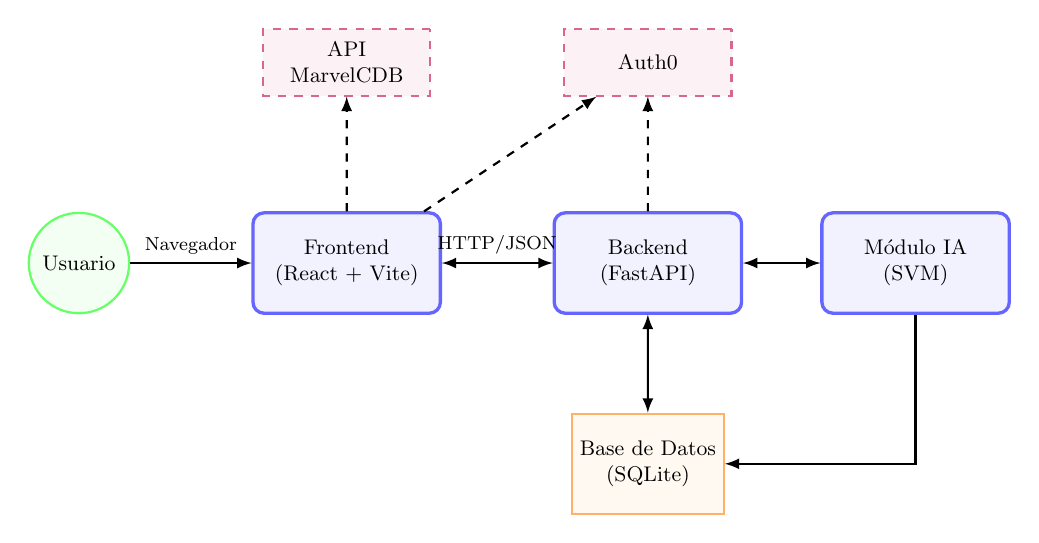
\begin{tikzpicture}[
        scale=0.85, transform shape,
        caja/.style={rectangle, draw=blue!60, fill=blue!5, very thick, rounded corners, align=center, minimum height=1.5cm, minimum width=2.8cm, font=\small},
        bd/.style={rectangle, draw=orange!60, fill=orange!5, thick, align=center, minimum height=1.5cm, minimum width=2cm, font=\small},
        externo/.style={rectangle, draw=purple!60, fill=purple!5, dashed, thick, align=center, minimum height=1cm, minimum width=2.5cm, font=\small},
        actor/.style={circle, draw=green!60, fill=green!5, thick, minimum size=1.5cm, align=center, font=\small},
        flecha/.style={->, >=latex, thick}
    ]
        \node[actor] (user) at (0,0) {Usuario};
        \node[caja] (front) at (4,0) {Frontend\\(React + Vite)};
        \node[caja] (back) at (8.5,0) {Backend\\(FastAPI)};
        \node[caja] (ia) at (12.5,0) {Módulo IA\\(SVM)};
        \node[bd] (db) at (8.5,-3) {Base de Datos\\(SQLite)};
        \node[externo] (marvel) at (4,3) {API\\MarvelCDB};
        \node[externo] (auth) at (8.5,3) {Auth0};

        \draw[flecha] (user) -- node[above, font=\footnotesize] {Navegador} (front);
        \draw[flecha, <->] (front) -- node[above, font=\footnotesize] {HTTP/JSON} (back);
        \draw[flecha, <->] (back) -- (ia);
        \draw[flecha, <->] (back) -- (db);
        \draw[flecha] (ia) |- (db);
        \draw[flecha, dashed] (front) -- (marvel);
        \draw[flecha, dashed] (front) -- (auth);
        \draw[flecha, dashed] (back) -- (auth);
    \end{tikzpicture}
    \caption{Arquitectura de alto nivel: frontend, backend y servicios externos.}
    \label{fig:arquitectura}
\end{figure}

A continuación se muestra la vista funcional del sistema mediante un diagrama de casos de uso: las acciones que el usuario puede realizar en AIForge, agrupadas en búsqueda y catálogo, partidas y recomendación, gestión de mazos, y las transversales (registro, perfil y contacto con soporte).

\begin{figure}[H]
    \centering
    \includegraphics[width=1\textwidth]{diagrama_casos_uso.png}
    \caption{Diagrama de Casos de Uso del sistema AIForge}
    \label{fig:casos_uso}
\end{figure}

% -----------------------------------------------------------------------------
\section{Diseño de la base de datos}
% -----------------------------------------------------------------------------

El modelo de datos se ha diseñado priorizando la integridad referencial y la consistencia. Se utiliza un esquema relacional en SQLite donde las entidades principales están vinculadas mediante claves foráneas con restricciones de borrado en cascada (\texttt{ON DELETE CASCADE}), de modo que al eliminar un usuario se eliminan sus mazos y partidas, y al eliminar un mazo se eliminan las partidas, comentarios y referencias en favoritos asociados.

\begin{figure}[H]
    \centering
    \includegraphics[width=1\textwidth]{diagrama_uml_bd.png}
    \caption{Diagrama de clases (Modelo Entidad-Relación) de la base de datos.}
    \label{fig:uml_bd}
\end{figure}

\subsection{Entidades principales}

A continuación se describen todas las entidades del modelo y su papel en el sistema.

\begin{itemize}
    \item \textbf{users}: Almacena la información de perfil de los usuarios autenticados (identificador Auth0, email, nombre, foto). El backend no gestiona contraseñas; la autenticación se delega en Auth0. Esta tabla es la base de la propiedad: todo mazo, partida o favorito se asocia a un \texttt{user\_id}.
    \item \textbf{cards}: Contiene el catálogo completo de cartas del juego (héroes, villanos, aliados, eventos, esquemas, etc.), importado desde la API de MarvelCDB. Incluye campos como \texttt{marvelcdb\_code} para identificación unívoca, \texttt{aspect}, \texttt{type\_code}, \texttt{deck\_limit} e \texttt{is\_unique}, necesarios para la validación de mazos y para referenciar el villano en cada partida.
    \item \textbf{card\_sets}: Almacena los sets de cartas (identificador, nombre, código y número de cartas). Es una tabla de soporte para la organización del catálogo; las cartas referencian conceptualmente estos sets mediante \texttt{pack\_code} y \texttt{pack\_name}.
    \item \textbf{decks}: Almacena los mazos creados por los usuarios o importados sin login. Guarda el nombre, la descripción, el héroe (nombre e ID), el aspecto y la lista de cartas en formato JSON. \texttt{user\_id} puede ser nulo en mazos importados sin autenticación. Esta entidad es central: las partidas y los favoritos dependen de ella.
    \item \textbf{game\_configurations}: Registra el histórico de partidas jugadas (usuario, mazo utilizado, dificultad, villano enfrentado, resultado y fecha). Es la fuente de verdad para el entrenamiento del modelo SVM: a partir de estas filas se extraen las características y la variable objetivo (victoria/derrota).
    \item \textbf{user\_favorites}: Gestiona la relación muchos a muchos entre usuarios y mazos marcados como favoritos. Evita duplicados mediante restricción \texttt{UNIQUE(user\_id, deck\_id)}. Permite listar «mis favoritos» y mostrar en el frontend si un mazo está marcado.
    \item \textbf{deck\_comments}: Almacena los comentarios de los usuarios sobre un mazo. Guarda el identificador del mazo, el autor (vía \texttt{auth0\_id}) y el texto. Permite editar y borrar solo al autor y se elimina en cascada si se borra el mazo.
\end{itemize}

Las tablas que tienen mayor influencia en el sistema (base de usuarios, catálogo de cartas, mazos y partidas) se detallan a continuación con su estructura.

\subsubsection{Tabla \texttt{users}}

Es la raíz de la propiedad en el sistema: cada mazo, partida y favorito está asociado a un usuario. El \texttt{auth0\_id} permite sincronizar con Auth0 sin almacenar contraseñas.

\begin{table}[H]
    \centering
    \small
    \begin{tabular}{|l|l|l|}
        \hline
        \textbf{Campo} & \textbf{Tipo} & \textbf{Descripción} \\
        \hline
        id & INTEGER PK & Identificador único interno \\
        auth0\_id & TEXT UNIQUE & Identificador del usuario en Auth0 \\
        email & TEXT UNIQUE & Correo electrónico \\
        name & TEXT & Nombre para mostrar \\
        picture\_url & TEXT & URL de la foto de perfil \\
        created\_at & TIMESTAMP & Fecha de alta \\
        updated\_at & TIMESTAMP & Última actualización \\
        \hline
    \end{tabular}
    \caption{Estructura de la tabla \texttt{users}. Base de la propiedad de mazos y partidas.}
    \label{tab:users}
\end{table}

\subsubsection{Tabla \texttt{cards}}

Contiene todo el catálogo de cartas (jugador y encounter). El campo \texttt{marvelcdb\_code} permite alinear con la API de MarvelCDB; \texttt{deck\_limit} e \texttt{is\_unique} se usan para validar la composición de los mazos. \texttt{villain\_id} en \texttt{game\_configurations} referencia \texttt{cards.id} para el villano enfrentado.

\begin{table}[H]
    \centering
    \small
    \begin{tabular}{|l|l|l|}
        \hline
        \textbf{Campo} & \textbf{Tipo} & \textbf{Descripción} \\
        \hline
        id & INTEGER PK & Identificador (compatible MarvelCDB) \\
        name & TEXT & Nombre de la carta \\
        aspect & TEXT & Clase (aggression, justice, leadership, etc.) \\
        type, type\_code & TEXT & Tipo (ally, event, villain, hero, etc.) \\
        cost & INTEGER & Coste en recursos \\
        pack\_code, pack\_name & TEXT & Pack de origen \\
        deck\_limit & INTEGER & Límite de copias por mazo \\
        is\_unique & BOOLEAN & Si la carta es única \\
        marvelcdb\_code & VARCHAR(20) & Código en MarvelCDB \\
        \hline
    \end{tabular}
    \caption{Estructura de la tabla \texttt{cards} (columnas principales). Base del catálogo y de las referencias villano/héroe.}
    \label{tab:cards}
\end{table}

\subsubsection{Tabla \texttt{decks}}

Almacena cada mazo con su composición en JSON (lista de cartas con cantidades). \texttt{hero\_id} referencia la carta del héroe en \texttt{cards}; \texttt{user\_id} puede ser NULL para mazos importados sin login. \texttt{is\_public} controla la visibilidad en listados públicos.

\begin{table}[H]
    \centering
    \small
    \begin{tabular}{|l|l|l|}
        \hline
        \textbf{Campo} & \textbf{Tipo} & \textbf{Descripción} \\
        \hline
        id & INTEGER PK & Identificador único \\
        name & TEXT & Nombre del mazo \\
        description & TEXT & Descripción opcional \\
        hero\_name & TEXT & Nombre del héroe (para mostrar) \\
        hero\_id & INTEGER & ID del héroe en \texttt{cards} \\
        aspect & TEXT & Aspecto (aggression, justice, etc.) \\
        cards & TEXT (JSON) & Lista de cartas con cantidades \\
        is\_public & BOOLEAN & Visible en listados públicos \\
        user\_id & INTEGER FK (nullable) & Propietario; NULL si importado sin login \\
        created\_at & TIMESTAMP & Fecha de creación \\
        updated\_at & TIMESTAMP & Última modificación \\
        \hline
    \end{tabular}
    \caption{Estructura de la tabla \texttt{decks}. Central para partidas, favoritos y comentarios.}
    \label{tab:decks}
\end{table}

\subsubsection{Tabla \texttt{game\_configurations}}

Cada fila es una partida jugada: quién jugó, con qué mazo, contra qué villano, en qué dificultad y con qué resultado. Es la fuente de datos para el entrenamiento del SVM (características y etiqueta win/loss).

\begin{table}[H]
    \centering
    \small
    \begin{tabular}{|l|l|l|}
        \hline
        \textbf{Campo} & \textbf{Tipo} & \textbf{Descripción} \\
        \hline
        id & INTEGER PK & Identificador único \\
        user\_id & INTEGER FK $\rightarrow$ users & Jugador \\
        deck\_id & INTEGER FK $\rightarrow$ decks & Mazo utilizado \\
        difficulty & TEXT & normal \textbar\ expert \\
        villain\_id & INTEGER FK $\rightarrow$ cards & Villano enfrentado \\
        result & TEXT & win \textbar\ loss \\
        played\_at & TEXT & Fecha y hora de la partida \\
        \hline
    \end{tabular}
    \caption{Estructura de la tabla \texttt{game\_configurations}. Fuente de verdad para el entrenamiento del modelo de IA.}
    \label{tab:game_configurations}
\end{table}

\subsubsection{Tabla \texttt{user\_favorites}}

Tabla de relación entre usuarios y mazos favoritos. La restricción \texttt{UNIQUE(user\_id, deck\_id)} evita marcar el mismo mazo más de una vez por usuario. Las claves foráneas con \texttt{ON DELETE CASCADE} mantienen la integridad al borrar un usuario o un mazo.

\begin{table}[H]
    \centering
    \small
    \begin{tabular}{|l|l|l|}
        \hline
        \textbf{Campo} & \textbf{Tipo} & \textbf{Descripción} \\
        \hline
        id & INTEGER PK & Identificador único \\
        user\_id & INTEGER FK $\rightarrow$ users & Usuario \\
        deck\_id & INTEGER FK $\rightarrow$ decks & Mazo favorito \\
        created\_at & TEXT & Fecha de marcado \\
        \hline
    \end{tabular}
    \caption{Estructura de la tabla \texttt{user\_favorites}. Relación muchos a muchos usuario--mazo.}
    \label{tab:user_favorites}
\end{table}

Las tablas \texttt{card\_sets} y \texttt{deck\_comments} completan el modelo: la primera para organizar el catálogo por sets; la segunda para los comentarios sobre mazos, con borrado en cascada al eliminar el mazo y autoría identificada por \texttt{auth0\_id} para permitir edición y borrado solo al autor.

% -----------------------------------------------------------------------------
\section{Estructura del frontend}
\label{sec:estructura-frontend}
% -----------------------------------------------------------------------------

\subsection{Arquitectura en capas}

El frontend se organiza en cuatro capas con flujo unidireccional:
\begin{itemize}
    \item \textbf{Presentación}: páginas y componentes React (\texttt{Header}, \texttt{Footer}, \texttt{Layout}, \texttt{ImportDeckModal}, \texttt{Toast}, \texttt{ProtectedRoute}).
    \item \textbf{Servicios}: \texttt{api.ts} (llamadas al backend) y \texttt{marvelcdbService.ts} (API MarvelCDB).
    \item \textbf{Contexto}: estado global, en especial \texttt{AuthContext} (usuario, login/logout).
    \item \textbf{Utilidades}: tipos TypeScript (\texttt{Deck}, \texttt{Card}, etc.), convertidor MarvelCDB a formato interno y funciones auxiliares.
\end{itemize}
La presentación usa servicios y contexto; los servicios llaman a las APIs. No se usa librería de estado global (Redux); el estado se gestiona en componentes y contexto.

\subsection{Estructura de la aplicación y rutas}

La aplicación es una SPA (React Router): una sola carga y navegación sin recarga. Todas las rutas comparten un \texttt{Layout} común (cabecera y pie). Las rutas que requieren usuario autenticado están envueltas por el componente \texttt{ProtectedRoute}, que redirige al login si no hay sesión. La Tabla~\ref{tab:rutas} resume las rutas principales y el tipo de acceso.

\begin{table}[H]
    \centering
    \small
    \begin{tabular}{|l|l|c|}
        \hline
        \textbf{Ruta} & \textbf{Descripción} & \textbf{Acceso} \\
        \hline
        \texttt{/} & Inicio, estadísticas & Público \\
        \texttt{/decks} & Lista de mazos & Público \\
        \texttt{/decks/:id} & Detalle de mazo & Público \\
        \texttt{/decks/:id/edit} & Editar mazo & Protegido \\
        \texttt{/mydecks} & Mis mazos & Protegido \\
        \texttt{/create-deck} & Crear mazo & Protegido \\
        \texttt{/configure-game} & Registrar partida & Protegido \\
        \texttt{/add-game} & Añadir partida (elegir/importar mazo) & Público \\
        \texttt{/favorites} & Favoritos & Protegido \\
        \texttt{/games-history} & Historial partidas & Público \\
        \texttt{/ai-recommendation} & Recomendación IA & Protegido \\
        \texttt{/cards}, \texttt{/cards/set/:id}, \texttt{/cards/search} & Cartas y búsqueda & Público \\
        \texttt{/faq} & Preguntas frecuentes & Público \\
        \texttt{/profile} & Perfil usuario & Protegido \\
        \hline
    \end{tabular}
    \caption{Rutas principales del frontend y tipo de acceso}
    \label{tab:rutas}
\end{table}

\subsection{Diseño de la interfaz de usuario}

Se ha optado por una interfaz responsive (Tailwind CSS): en escritorio la cabecera muestra menú horizontal; en móvil, menú hamburguesa. Los listados (mazos, cartas) se muestran en rejillas adaptativas. Todas las páginas comparten \texttt{Layout}, \texttt{Header} y \texttt{Footer} para una navegación consistente. El feedback al usuario se hace con toasts (éxito, error, información) y con diálogos de confirmación en acciones destructivas; los formularios validan antes de enviar a la API.

% -----------------------------------------------------------------------------
\section{Diseño del sistema de recomendación (IA)}
% -----------------------------------------------------------------------------

El módulo de Inteligencia Artificial se ha diseñado para resolver un problema de clasificación binaria: predecir si una combinación de mazo y héroe resultará en victoria o derrota contra un villano específico.

\subsection{Modelo y características}

Se ha seleccionado un modelo de \textbf{Máquinas de Vectores de Soporte (SVM)} con kernel radial (RBF). Este algoritmo es adecuado para encontrar fronteras de decisión complejas en espacios de características cuando el número de muestras puede ser limitado.

El modelo no utiliza las cartas individuales como entrada directa para evitar una dimensionalidad excesiva. En su lugar, se extraen \textbf{características agregadas} por partida, tales como:
\begin{itemize}
    \item Identificador del héroe y aspecto del mazo (aggression, justice, leadership, protection, pool).
    \item Identificador del villano y dificultad (normal/expert).
    \item Coste medio de las cartas del mazo.
    \item Proporción de tipos de carta (eventos, aliados, mejoras, apoyos).
\end{itemize}
La variable objetivo es el resultado de la partida (victoria o derrota) almacenado en \texttt{game\_configurations.result}.

\subsection{Flujo de datos}

El sistema opera en dos modos: entrenamiento asíncrono y predicción en tiempo real.

\begin{enumerate}
    \item \textbf{Entrenamiento:} Cuando se registran nuevas partidas, un proceso en segundo plano (BackgroundTasks) extrae los datos de \texttt{game\_configurations} y \texttt{decks}, recalcula las características y reentrena el modelo SVM, persistiendo el resultado en disco (\texttt{.pkl}) en la ruta configurada por la variable de entorno \texttt{MODEL\_PATH}.
    \item \textbf{Recomendación:} Ante una solicitud del usuario (villano y dificultad), el sistema carga el modelo entrenado, evalúa las combinaciones héroe--aspecto según la probabilidad de victoria y genera mazos completos eligiendo cartas coherentes con el aspecto y las reglas del juego. Si no hay modelo (pocos datos), se utiliza un criterio determinista de respaldo.
\end{enumerate}

\begin{figure}[H]
    \centering
    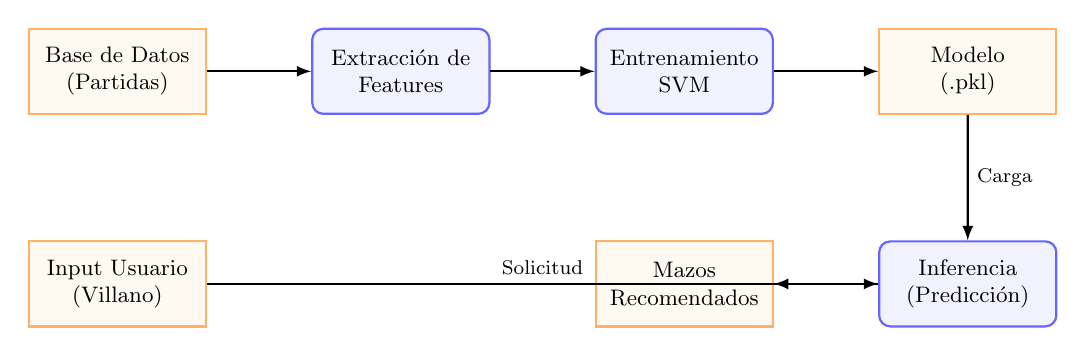
\begin{tikzpicture}[
        scale=0.9, transform shape,
        caja/.style={rectangle, draw=blue!60, fill=blue!5, thick, align=center, minimum height=1.2cm, minimum width=2.5cm, rounded corners, font=\small},
        dato/.style={rectangle, draw=orange!60, fill=orange!5, thick, align=center, minimum height=1.2cm, minimum width=2.5cm, font=\small},
        flecha/.style={->, >=latex, thick}
    ]
        \node[dato] (db) at (0,3) {Base de Datos\\(Partidas)};
        \node[caja] (prep) at (4,3) {Extracción de\\Features};
        \node[caja] (train) at (8,3) {Entrenamiento\\SVM};
        \node[dato] (model) at (12,3) {Modelo\\(.pkl)};
        \node[dato] (input) at (0,0) {Input Usuario\\(Villano)};
        \node[caja] (infer) at (12,0) {Inferencia\\(Predicción)};
        \node[dato] (output) at (8,0) {Mazos\\Recomendados};

        \draw[flecha] (db) -- (prep);
        \draw[flecha] (prep) -- (train);
        \draw[flecha] (train) -- (model);
        \draw[flecha] (input) -- node[above, font=\footnotesize] {Solicitud} (infer);
        \draw[flecha] (model) -- node[right, font=\footnotesize] {Carga} (infer);
        \draw[flecha] (infer) -- (output);
    \end{tikzpicture}
    \caption{Flujo del sistema de recomendación: entrenamiento e inferencia.}
    \label{fig:flujo_svm}
\end{figure}

% -----------------------------------------------------------------------------
\section{Herramientas utilizadas}
% -----------------------------------------------------------------------------

Durante el desarrollo y despliegue del sistema se han utilizado diversas herramientas que han facilitado la programación, la integración, las pruebas y la publicación.

\subsection{Backend}

\begin{itemize}
    \item \textbf{Python y FastAPI:} El backend está construido con Python 3.11 y FastAPI. Se eligió por su alto rendimiento, validación automática de datos con Pydantic y generación de documentación Swagger. El servidor ASGI utilizado es Uvicorn.
    \item \textbf{SQLite:} Motor de base de datos relacional ligero y portable, ideal para el volumen de datos del proyecto y su despliegue mediante volúmenes persistentes en Render.
    \item \textbf{scikit-learn:} Librería utilizada para la implementación, entrenamiento y validación del modelo de Máquinas de Vectores de Soporte (SVM), incluyendo la división entrenamiento/prueba y la serialización del modelo con \texttt{pickle}.
    \item \textbf{Postman:} Herramienta empleada para la prueba y validación manual de todos los endpoints de la API REST antes de su integración con el frontend (incluyendo cabecera \texttt{X-Auth0-ID} y cuerpos JSON).
\end{itemize}

\subsection{Frontend}

\begin{itemize}
    \item \textbf{Visual Studio Code:} IDE utilizado para el desarrollo del frontend (React y TypeScript), con extensiones como ESLint, Prettier y GitLens e integración directa con Git y GitHub.
    \item \textbf{React y TypeScript:} Biblioteca principal para la construcción de la interfaz de usuario, potenciada con el tipado estático de TypeScript para reducir errores en tiempo de ejecución.
    \item \textbf{Vite:} Herramienta de construcción (\textit{bundler}) utilizada por su velocidad en el servidor de desarrollo y eficiencia en el empaquetado para producción.
    \item \textbf{Tailwind CSS:} Framework de utilidades CSS que ha permitido un diseño rápido, consistente y totalmente responsive (móvil y escritorio).
    \item \textbf{Auth0 (cliente):} SDK para React (\texttt{@auth0/auth0-react}) para login, registro y proveedores sociales; el frontend redirige a Auth0 y el backend identifica al usuario mediante la cabecera \texttt{X-Auth0-ID}.
\end{itemize}

\subsection{Infraestructura y servicios}

\begin{itemize}
    \item \textbf{Auth0:} Servicio externo delegado para la gestión segura de identidades (registro y login). El backend recibe el \texttt{auth0\_id} en cabecera y mantiene la tabla \texttt{users} sincronizada sin almacenar contraseñas.
    \item \textbf{API MarvelCDB:} API pública utilizada para la importación del catálogo de cartas y sets, y para completar cartas faltantes mediante los endpoints \texttt{check-missing} e \texttt{import-missing}.
    \item \textbf{Render:} Plataforma PaaS utilizada para el despliegue del backend, con disco persistente en \texttt{/data} para la base de datos SQLite y el archivo del modelo (\texttt{DB\_PATH}, \texttt{MODEL\_PATH}).
    \item \textbf{Vercel:} Plataforma utilizada para el despliegue y distribución global del frontend estático.
    \item \textbf{Git y GitHub:} Sistema de control de versiones y repositorio remoto para la gestión del código fuente, el historial de cambios y el despliegue automático en Render.
\end{itemize}
